\let\negmedspace\undefined
\let\negthickspace\undefined
\documentclass[journal,12pt,onecolumn]{IEEEtran}
\usepackage{cite}
\usepackage{amsmath,amssymb,amsfonts,amsthm}
\usepackage{algorithmic}
\usepackage{graphicx}
\usepackage{textcomp}
\usepackage{xcolor}
\usepackage{txfonts}
\usepackage{listings}
\usepackage{enumitem}
\usepackage{mathtools}
\usepackage{gensymb}
\usepackage{comment}
\usepackage[breaklinks=true]{hyperref}
\usepackage{tkz-euclide} 
\usepackage{gvv}                                        
%\def\inputGnumericTable{}                                 
\usepackage[latin1]{inputenc}     
\usepackage{xparse}
\usepackage{color}                                            
\usepackage{array}                                            
\usepackage{longtable}                                       
\usepackage{calc}                                             
\usepackage{multirow}
\usepackage{multicol}
\usepackage{hhline}                                           
\usepackage{ifthen}                                           
\usepackage{lscape}
\usepackage{tabularx}
\usepackage{array}
\usepackage{float}
\newtheorem{theorem}{Theorem}[section]
\newtheorem{problem}{Problem}
\newtheorem{proposition}{Proposition}[section]
\newtheorem{lemma}{Lemma}[section]
\newtheorem{corollary}[theorem]{Corollary}
\newtheorem{example}{Example}[section]
\newtheorem{definition}[problem]{Definition}
\newcommand{\BEQA}{\begin{eqnarray}}
\newcommand{\EEQA}{\end{eqnarray}}
\newcommand{\define}{\stackrel{\triangle}{=}}
\theoremstyle{remark}
\newtheorem{rem}{Remark}
% Marks the beginning of the document
\begin{document}
\title{gate 1}
\author{AI25btech11022 - Narshitha}
\maketitle
\renewcommand{\thefigure}{\theenumi}
\renewcommand{\thetable}{\theenumi}
\begin{center}
\large \textbf{2019}\\
\large \textbf{CS:Computer science and Engineering}\\
\end{center}

\begin{enumerate}
   



\item The expenditure on the project \_\_\_\_\_ as follows: equipment Rs.20 lakhs, salaries Rs.12 lakhs, and contingency Rs.3 lakhs.\hfill \textbf{(GATE EE 2025)}

\begin{enumerate}
\item  break down
\item  break
\item  breaks down
\item  breaks
\end{enumerate}

\item The search engine's business model \_\_\_\_\_ around the fulcrum of trust.\hfill \textbf{(GATE EE 2025)}

\begin{enumerate}
\item  revolves
\item  plays
\item  sinks
\item  bursts
\end{enumerate}

\item Two cars start at the same time from the same location and go in the same direction. 
The speed of the first car is 50 km/h and the speed of the second car is 60 km/h. 
The number of hours it takes for the distance between the two cars to be 20 km is \_\_\_.
\hfill \textbf{(GATE EE 2025)}
\begin{enumerate}
\item  1
\item  2
\item  3
\item  6
\end{enumerate}

\item Ten friends planned to share equally the cost of buying a gift for their teacher. 
When two of them decided not to contribute, each of the other friends had to pay Rs.150 more. 
The cost of the gift was Rs. \_\_\_. \hfill \textbf{(GATE EE 2025)}

\begin{enumerate}
\item  666
\item  3000
\item  6000
\item 12000
\end{enumerate}

\item A court is to a judge as \_\_\_ is to a teacher.\hfill \textbf{(GATE EE 2025)}

\begin{enumerate}
\item  a student
\item  a punishment
\item  a syllabus
\item  a school
\end{enumerate}

\item The police arrested four criminals - P, Q, R and S. The criminals knew each other. 
They made the following statements:


P says "Q committed the crime."\\
 Q says "S committed the crime."\\
 R says "I did not do it."\\
 S says "What Q said about me is false."\\


Assume only one of the arrested four committed the crime and only one of the statements made above is true.  
Who committed the crime? \hfill \textbf{(GATE EE 2025)}

\begin{enumerate}
\item  P
\item  R
\item  S
\item  Q
\end{enumerate}

\item In the given diagram, teachers are represented in the triangle, researchers in the circle and administrators in the rectangle. Out of the total number of the people, the percentage of administrators shall be in the range of \_\_\_.\hfill \textbf{(GATE EE 2025)}
\begin{figure}[H]
    \centering
    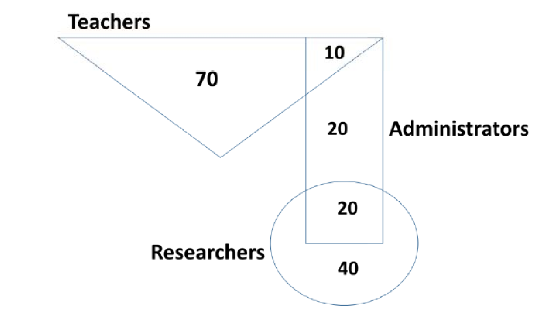
\includegraphics[width=0.5\linewidth]{figs/fig1.png}
    \caption{ }
    \label{fig1}
\end{figure}
\begin{enumerate}
\item  0 to 15
\item  16 to 30
\item  31 to 45
\item  46 to 60
\end{enumerate}

\item A recent High Court judgement has sought to dispel the idea of begging as a disease - which leads to its stigmatization and criminalization - and to regard it as a symptom. The underlying disease is the failure of the state to protect citizens who fall through the social security net.

Which one of the following statements can be inferred from the given passage?\hfill \textbf{(GATE EE 2025)}

\begin{enumerate}
\item  Beggars are lazy people who beg because they are unwilling to work
\item  Beggars are created because of the lack of social welfare schemes
\item  Begging is an offence that has to be dealt with firmly
\item  Begging has to be banned because it adversely affects the welfare of the state
\end{enumerate}

\item In a college, there are three student clubs. Sixty students are only in the Drama club, 80 students are only in the Dance club, 30 students are only in the Maths club, 40 students are in both Drama and Dance clubs, 12 students are in both Dance and Maths clubs, 7 students are in both Drama and Maths clubs, and 2 students are in all the clubs. If 75\% of the students in the college are not in any of these clubs, then the total number of students in the college is \_\_\_. \hfill \textbf{(GATE EE 2025)}
\begin{enumerate}
    \item 1000
    \item 975
    \item 900
    \item 225
\end{enumerate}
\item Three of the five students allocated to a hostel put in special requests to warden . Given the floor plan of the vacant rooms ,select the allocation plan that will accomodate all their requests.\\
Request by X: Due to pollen allergy I want to avoid a wing next to the garden \\
Request by Y: I want to live as far from the washroom since I am very sensitive to smell\\
Request by Z:I belive in vasthu and so want to stay in the south-west wing \\
The shaded room are already occupied. WR is washroom \hfill \textbf{(GATE EE 2025)}
\begin{figure}[H]
    \centering
    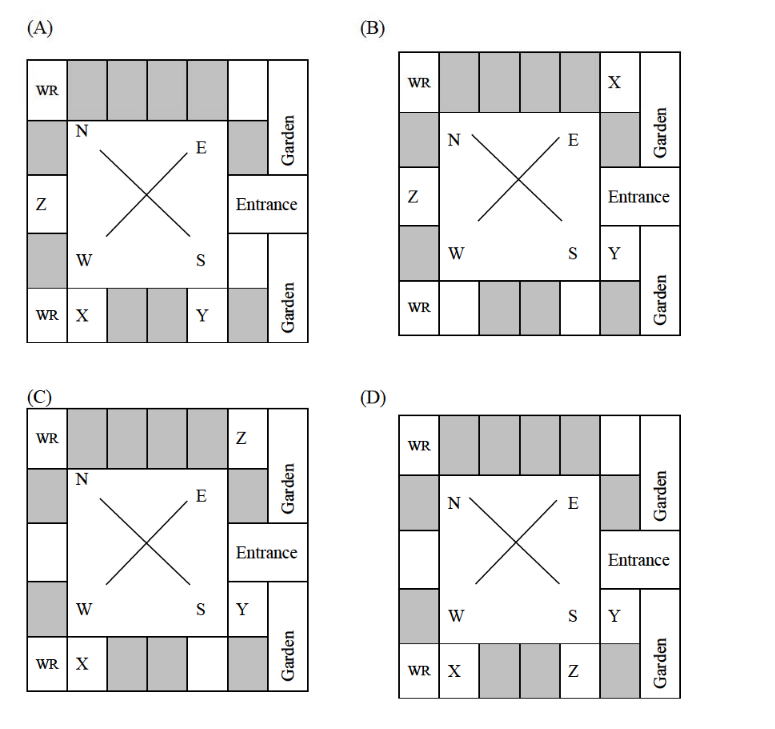
\includegraphics[width=0.5\linewidth]{figs/fig2.png}
    \caption{ }
    \label{fig2}
\end{figure}

\item A certain processor uses a fully associative cache of size 16 kB. The cache block size is 16 bytes. Assume that the main memory is byte addressable and uses a 32-bit address. How many bits are required for the \textit{Tag} and the \textit{Index} fields respectively in the addresses generated by the processor? \hfill \textbf{(GATE EE 2025)}

\begin{enumerate} 
\item 24 bits and 0 bits
\item 28 bits and 4 bits
\item 24 bits and 4 bits
\item 28 bits and 0 bits
\end{enumerate}

\item The chip select logic for a certain DRAM chip in a memory system design is shown below. Assume that the memory system has 16 address lines denoted by $A_{15}$ to $A_{0}$. What is the range of addresses (in hexadecimal) of the memory system that can get enabled by the chip select (CS) signal?\hfill \textbf{(GATE EE 2025)}
\begin{figure}[H]
    \centering
    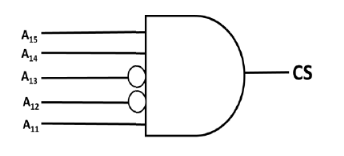
\includegraphics[width=0.5\linewidth]{figs/fig3.png}
    \caption{ }
    \label{fig3}
\end{figure}
\begin{enumerate} 
\item C800 to CFFF
\item CA00 to CAFF
\item C800 to C8FF
\item DA00 to DFFF
\end{enumerate}

\item Which one of the following kinds of derivation is used by LR parsers?
\hfill \textbf{(GATE EE 2025)}
\begin{enumerate} 
\item Leftmost
\item Leftmost in reverse
\item Rightmost
\item Rightmost in reverse
\end{enumerate}

\item In 16-bit 2's complement representation, the decimal number $-28$ is:\hfill \textbf{(GATE EE 2025)}

\begin{enumerate} 
\item 1111 1111 1110 0100
\item 0000 0000 1110 0100
\item 1111 1111 1110 0100
\item 1000 0000 1110 0100
\end{enumerate}

\item Let $U = \{1,2,\ldots,n\}$. Let $A = \{(X,Y) \mid X \in X, X \subseteq U\}$. Consider the following two statements on $|A|$.   
\begin{enumerate}
\item I. $|A| = n2^{n-1}$
\item II. $|A| = \sum_{k=1}^n k\binom{n}{k}$
\end{enumerate}
Which of the above statements is/are TRUE?\hfill \textbf{(GATE EE 2025)}

\begin{enumerate} 
\item Only I
\item Only II
\item Both I and II
\item Neither I nor II
\end{enumerate}

\item Which one of the following is NOT a valid identity?\hfill \textbf{(GATE EE 2025)}

\begin{enumerate} 
\item $(x \oplus y) \oplus z = x \oplus (y \oplus z)$
\item $(x + y) \oplus z = x \oplus (y + z)$
\item $x \otimes y = x+y$, if $x=y=0$
\item $x \oplus y = (x'y + xy')$
\end{enumerate}

\item If $L$ is a regular language over $\Sigma = \{a,b\}$, which one of the following languages is NOT regular?\hfill \textbf{(GATE EE 2025)}

\begin{enumerate} 
\item $L \cdot L^R = \{xy \mid x \in L, y^R \in L\}$
\item $\{ww^R \mid w \in L\}$
\item $\text{Prefix}(L) = \{x \in \Sigma^* \mid \exists y \in \Sigma^* \text{ such that } xy \in L\}$
\item $\text{Suffix}(L) = \{y \in \Sigma^* \mid \exists x \in \Sigma^* \text{ such that } xy \in L\}$
\end{enumerate}

\item Consider $Z = X - Y$, where $X, Y$ and $Z$ are all in sign-magnitude form. $X$ and $Y$ are each represented in $n$ bits. To avoid overflow, the representation of $Z$ would require a minimum of:\hfill \textbf{(GATE EE 2025)}

\begin{enumerate} 
\item n bits
\item n - 1 bits
\item n + 1 bits
\item n + 2 bits
\end{enumerate}

\item Let $X$ be a square matrix. Consider the following two statements on $X$.  \\

I.$X$ is invertible.  \\
II. Determinant of $X$ is non-zero.  \\

Which one of the following is TRUE? \hfill \textbf{(GATE EE 2025)}

\begin{enumerate} 
\item I implies II; II does not imply I.
\item II implies I; I does not imply II.
\item I does not imply II; II does not imply I.
\item I and II are equivalent statements.
\end{enumerate}

\item Let $G$ be an arbitrary group. Consider the following relations on $G$:  
\[
R_1: \forall a,b \in G, \ a \,R_1\, b \text{ if and only if } \exists g \in G \text{ such that } a = g^{-1} b g
\]  
\[
R_2: \forall a,b \in G, \ a \,R_2\, b \text{ if and only if } a = b^{-1}
\]
Which of the above is/are equivalence relation/relations? \hfill \textbf{(GATE EE 2025)}
 
\begin{enumerate}
    \item  $R_1$ and $R_2$
    \item  $R_1$ only
    \item  $R_2$ only
    \item  Neither $R_1$ nor $R_2$
\end{enumerate}

 

\item  Consider the following two statements about database transaction schedules:  \\
1. Strict two-phase locking protocol generates conflict serializable schedules that are also recoverable.\\
2. Timestamp-ordering concurrency control protocol with Thomas' Write Rule can generate view serializable schedules that are not conflict serializable.\\
Which of the above statements is/are TRUE?  \hfill \textbf{(GATE EE 2025)}

\begin{enumerate}
    \item  I only
    \item  II only
    \item  Both I and II
    \item  Neither I nor II
\end{enumerate}

 

\item  Let $G$ be an undirected complete graph on $n$ vertices, where $n > 2$. Then, the number of different Hamiltonian cycles in $G$ is equal to  \hfill \textbf{(GATE EE 2025)}
\begin{enumerate}
    \item  $n!$
    \item  $(n-1)!$
    \item  $1$
    \item  $\dfrac{(n-1)!}{2}$
\end{enumerate}

 

\item Compute  
\[
\lim_{x \to 3} \frac{x^4 - 81}{2x^2 - 5x - 3}
\] \hfill \textbf{(GATE EE 2025)}
\begin{enumerate}
    \item  $1$
    \item  $\dfrac{53}{12}$
    \item  $\dfrac{108}{7}$
    \item  Limit does not exist
\end{enumerate}

 

\item  Which one of the following statements is NOT correct about the B+ tree data structure used for creating an index of a relational database table?\hfill \textbf{(GATE EE 2025)}  
\begin{enumerate}
    \item  B+ Tree is a height-balanced tree
    \item  Non-leaf nodes have pointers to data records
    \item  Key values in each node are kept in sorted order
    \item  Each leaf node has a pointer to the next leaf node
\end{enumerate}

 

\item  For $\Sigma = \{a,b\}$, let us consider the regular language 
\[
L = \{ \, x \mid x = a^{2+3k} \text{ or } x = b^{10+12k}, \, k \geq 0 \, \}
\]
Which one of the following can be a pumping length (the constant guaranteed by the pumping lemma) for $L$? \hfill \textbf{(GATE EE 2025)} 
\begin{enumerate}
    \item  3
    \item  5
    \item  9
    \item  24
\end{enumerate}


\item  Which of the following protocol pairs can be used to send and retrieve e-mails (in that order)?  \hfill \textbf{(GATE EE 2025)}
\begin{enumerate}
    \item  IMAP, POP3
    \item  SMTP, POP3
    \item  SMTP, MIME
    \item  IMAP, SMTP
\end{enumerate}

\item  The following C program is executed on a Unix/Linux system:
\begin{verbatim}[language=C]
#include <unistd.h>
int main()
{
    int i;
    for (i = 0; i < 10; i++)
        if (i & 2 == 0) fork();
    return 0;
}
\end{verbatim}

The total number of child processes created is \underline{\hspace{3cm}}. \\[1em]
\hfill \textbf{(GATE EE 2025)}

\item  Consider the following C program:
\begin{verbatim}[language=C]
#include <stdio.h>
int jumble(int x, int y) {
    x = 2 * x + y;
    return x;
}
int main() {
    int x = 2, y = 5;
    y = jumble(y, x);
    x = jumble(y, x);
    printf("%d \n", x);
    return 0;
}
\end{verbatim}

The value printed by the program is \underline{\hspace{3cm}}. \\[1em]
\hfill \textbf{(GATE EE 2025)}

\item  Consider the grammar given below:
\[
S \to Aa \quad 
A \to BD \quad 
B \to b \mid c \quad 
D \to d \mid \epsilon
\]

Let $a, b, d, \$$ be indexed as follows:
\begin{center}
    


\begin{tabular}{|c|c|c|c|}
 
\hline
a & b & d & \$ \\
\hline
3 & 2 & 1 & 0 \\
\hline
\end{tabular}\\
\end{center}
Compute the FOLLOW set of the non-terminal $B$ and write the index values for the symbols in the FOLLOW set in the descending order. (For example, if the FOLLOW set is $\{a, b, d, \$\}$, then the answer should be $3210$.) 
\hfill \textbf{(GATE EE 2025)}
\item  An array of 25 distinct elements is to be sorted using quicksort. Assume that the pivot element is chosen uniformly at random. The probability that the pivot element gets placed in the worst possible location in the first round of partitioning (rounded off to 2 decimal places) is \underline{\hspace{3cm}}. \\[1em]
\hfill \textbf{(GATE EE 2025)}
\item  The value of $3^{51} \bmod 5$ is \underline{\hspace{3cm}}. \\[1em]

\hfill \textbf{(GATE EE 2025)}
\item  Two numbers are chosen independently and uniformly at random from the set $\{1, 2, \dots, 13\}$. The probability (rounded off to 3 decimal places) that their 4-bit (unsigned) binary representations have the same most significant bit is \underline{\hspace{3cm}}. \\[1em]

\hfill \textbf{(GATE EE 2025)}
\item Consider three concurrent processes $P_1, P_2$ and $P_3$ as shown below, which access a shared variable $D$ that has been initialized to 100.\\
\begin{center}
    


\begin{tabular}{|c|c|c|}
\hline
P1 & P2 & P3 \\
\hline
D = D + 20 & D = D - 50 & D = D + 10 \\
\vdots & \vdots & \vdots \\
\hline
\end{tabular}

\end{center}
The processes are executed on a uniprocessor system running a time-shared operating system. If the minimum and maximum possible values of $D$ after the three processes have completed execution are $X$ and $Y$ respectively, then the value of $Y - X$ is \underline{\hspace{3cm}}. \\

\hfill \textbf{(GATE EE 2025)}
\item Consider the following C program:
\begin{verbatim}
#include <stdio.h>
int main(){
    int arr[]={1,2,3,4,5,6,7,8,9,0,1,2,5}, *ip=arr+4;
    printf("%d\n", ip[1]);
    return 0;
}
\end{verbatim}

The number that will be displayed on execution of the program is \_\_\_\_\_\_\_.
\hfill \textbf{(GATE EE 2025)}


\item  Consider a sequence of 14 elements: 
\[
A = [-5,-10,6,3,-1,-2,13,4,-9,-1,4,12,-3,0]
\]

The subsequence sum 
\[
S(i,j) = \sum_{k=i}^{j} A[k].
\]
Determine the maximum of $S(i,j)$, where $0 \leq i \leq j < 14$. (Divide and conquer approach may be used.)
\hfill \textbf{(GATE EE 2025)}
\textbf{Answer:} \_\_\_\_\_\_\_.



\item Consider the following C function:
\begin{verbatim}
void convert(int n){
    if(n<0)
        printf("%d",n);
    else {
        convert(n/2);
        printf("%d",n&2);
    }
}
\end{verbatim}

Which one of the following will happen when the function convert is called with any positive integer $n$ as argument?\hfill \textbf{(GATE EE 2025)}

\begin{enumerate}
\item  It will print the binary representation of $n$ and terminate
\item  It will print the binary representation of $n$ in the reverse order and terminate
\item  It will print the binary representation of $n$ but will not terminate
\item  It will not print anything and will not terminate
\end{enumerate}



\item  Consider the following C program:
\begin{verbatim}
#include <stdio.h>
int r(){
    static int num = 7;
    return num--;
}

int main(){
    for(r(); r(); r())
        printf("%d",r());
    return 0;
}
\end{verbatim}

Which one of the following values will be displayed on execution of the program?
\hfill \textbf{(GATE EE 2025)}
\begin{enumerate}
\item  41
\item  52
\item  63
\item  630
\end{enumerate}



\item Consider three machines M, N, and P with IP addresses 
100.10.5.2, 100.10.5.5, and 100.10.5.6 respectively.  
The subnet mask is set to 255.255.255.252 for all the three machines.  
Which one of the following is true?\hfill \textbf{(GATE EE 2025)}

\begin{enumerate}
\item  M, N, and P all belong to the same subnet
\item  Only M and N belong to the same subnet
\item  Only N and P belong to the same subnet
\item  M, N, and P belong to three different subnets
\end{enumerate}


\item  Suppose that in an IP-over-Ethernet network, a machine $X$ wishes to find the MAC address of another machine $Y$ in its subnet. Which one of the following techniques can be used for this?  \hfill \textbf{(GATE EE 2025)}

\begin{enumerate}
  \item   $X$ sends an ARP request packet to the local gateway's IP address which then finds the MAC address of $Y$ and sends to $X$
  \item   $X$ sends an ARP request packet to the local gateway's MAC address which then finds the MAC address of $Y$ and sends to $X$
  \item   $X$ sends an ARP request packet with broadcast MAC address in its local subnet
  \item   $X$ sends an ARP request packet with broadcast IP address in its local subnet
\end{enumerate}


\item  Consider three 4-variable functions $f_1, f_2, f_3$ which are expressed in sum-of-minterms as  
\[
f_1 = \Sigma (0,2,5,8,14), \quad 
f_2 = \Sigma (2,3,6,8,14,15), \quad 
f_3 = \Sigma (2,7,11,14).
\]  
\begin{figure}
    \centering
    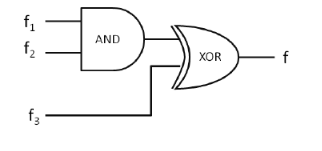
\includegraphics[width=0.5\linewidth]{figs/fig4.png}
    \caption{ }
    \label{fig4}
\end{figure}
For the following circuit with one AND gate and one XOR gate, the output function $f$ can be expressed as:  \hfill \textbf{(GATE EE 2025)}

\begin{enumerate}
  \item   $\Sigma (7,8,11)$
  \item   $\Sigma (2,7,8,11,14)$
  \item   $\Sigma (2,14)$
  \item   $\Sigma (0,2,3,5,6,7,8,11,14,15)$
\end{enumerate}



\item  Which one of the following languages over $\Sigma = \{a,b\}$ is \textbf{NOT} context-free?  \hfill \textbf{(GATE EE 2025)}

\begin{enumerate}
  \item   $\{ww^R \mid w \in \{a,b\}^*\}$
  \item   $\{w a^n b^n w^R \mid w \in \{a,b\}^*, n \geq 0\}$
  \item   $\{w a^n w^R b^n \mid w \in \{a,b\}^*, n \geq 0\}$
  \item   $\{a^i b^j \mid i \in \{n,3n,5n\}, n \geq 0\}$
\end{enumerate}

\item  Let the set of functional dependencies $F = \{QR \to S, R \to P, S \to Q\}$ hold on a relation schema $X = (PQRS)$. $X$ is not in BCNF. Suppose $X$ is decomposed into two schemas $Y$ and $Z$, where $Y = (PR)$ and $Z = (QRS)$.  

Consider the two statements given below.  

I. Both $Y$ and $Z$ are in BCNF  \\
II. Decomposition of $X$ into $Y$ and $Z$ is dependency preserving and lossless \\  

Which of the above statements is/are correct?\hfill \textbf{(GATE EE 2025)}  

\begin{enumerate}
  \item   Both I and II
  \item   I only
  \item   II only
  \item   Neither I nor II
\end{enumerate}

\item  Assume that in a certain computer, the virtual addresses are 64 bits long and the physical addresses are 48 bits long. The memory is word addressable. The page size is 8 KB and the word size is 8 bytes. The Translation Look-aside Buffer (TLB) in the address translation path has 128 valid entries. At most how many distinct virtual addresses can be translated without any TLB miss?  \hfill \textbf{(GATE EE 2025)}

\begin{enumerate}
  \item   $16 \times 2^{10}$\hfill \textbf{(GATE EE 2025)}
  \item   $256 \times 2^{10}$
  \item   $4 \times 2^{20}$
  \item   $8 \times 2^{20}$
\end{enumerate}


\item  Consider the following sets:  

S1. Set of all recursively enumerable languages over the alphabet $\{0,1\}$ \\
S2. Set of all syntactically valid C programs\\
S3. Set of all languages over the alphabet $\{0,1\}$ \\
S4. Set of all non-regular languages over the alphabet $\{0,1\}$ \\

Which of the above sets are uncountable?  \hfill \textbf{(GATE EE 2025)}

\begin{enumerate}
  \item   S1 and S2
  \item   S3 and S4\hfill \textbf{(GATE EE 2025)}
  \item   S2 and S3
  \item   S1 and S4
\end{enumerate}


\item  Consider the first order predicate formula $\varphi$:  
\[
\forall x \, [(\forall z \, z|x \Rightarrow (z = x) \lor (z = 1)) \Rightarrow \exists w \, (w > x) \land (\forall z \, z|w \Rightarrow (w = z) \lor (z = 1))].
\]  
Here ``$a|b$'' denotes that $a$ divides $b$, where $a$ and $b$ are integers. Consider the following sets:  

S1. $\{1,2,3,\ldots,100\}$ \\
S2. Set of all positive integers \\
S3. Set of all integers\\

Which of the above sets satisfy $\varphi$?  \hfill \textbf{(GATE EE 2025)}

\begin{enumerate}
  \item   S1 and S2
  \item   S1 and S3
  \item   S2 and S3
  \item   S1, S2 and S3\hfill \textbf{(GATE EE 2025)}
\end{enumerate}
\item Consider the following grammar and the semantic actions to support the inherited type declaration attributes. Let $X_1, X_2, X_3, X_4, X_5,$ and $X_6$ be the placeholders for the non-terminals $D, T, L$ or $L1$ in the following table:


\[
\begin{array}{|c|c|}
\hline
\text{Production rule} & \text{Semantic action} \\
\hline
D \to T \ L & X_1.\text{type} = X_2.\text{type} \\
T \to \text{int} & T.\text{type} = \text{int} \\
T \to \text{float} & T.\text{type} = \text{float} \\
L \to L1 , \ \text{id} & X_3.\text{type} = X_4.\text{type};\ \text{addType(id.entry, X}_5.\text{type)} \\
L \to \text{id} & \text{addType(id.entry, X}_6.\text{type)} \\
\hline
\end{array}
\]


Which one of the following are the appropriate choices for $X_1, X_2, X_3$, and $X_4$?
\hfill \textbf{(GATE EE 2025)}
\begin{enumerate}
\item  $X_1 = L, X_2 = T, X_3 = L1, X_4 = L$
\item  $X_1 = T, X_2 = L, X_3 = L1, X_4 = T$
\item  $X_1 = L, X_2 = L, X_3 = L1, X_4 = T$
\item  $X_1 = T, X_2 = L, X_3 = T, X_4 = L$
\end{enumerate}

\item There are $n$ unsorted arrays: $A_1, A_2, \dots, A_n$. Assume that $n$ is odd. Each of $A_1, A_2, \dots, A_n$ contains $n$ distinct elements. There are no common elements between any two arrays. The worst-case time complexity of computing the median of the medians of $A_1, A_2, \dots, A_n$ is \hfill \textbf{(GATE EE 2025)}
\begin{enumerate}
\item  $O(n)$
\item  $O(n \log n)$
\item  $O(n^2)$
\item  $\Omega(n^2 \log n)$
\end{enumerate}

\item Let $G$ be any connected, weighted, undirected graph.\\

I. $G$ has a minimum spanning tree, in which, if no two edges of $G$ have the same weight.\\
II. If $G$ has a unique minimum spanning tree, $H$, for every cut of $G$, there is a unique minimum-weight edge crossing the cut.\\


Which of the above two statements is/are TRUE?\hfill \textbf{(GATE EE 2025)}
\begin{enumerate}
\item  I only
\item  II only
\item  Both I and II
\item  Neither I nor II
\end{enumerate}

\item Consider the following snapshot of a system running $n$ concurrent processes. Process $i$ is holding $X_i$ instances of a resource $R$, $1 \leq i \leq n$. Assume that all instances of $R$ are currently in use. Further, for all $i$, process $i$ can place a request for at most $Y_i$ additional instances of $R$ while holding the $X_i$ instances it already has. Of the $n$ processes, there are exactly two processes $p$ and $q$ such that $Y_p = Y_q = 0$. Which one of the following conditions guarantees that no other process apart from $p$ and $q$ can complete execution? \hfill \textbf{(GATE EE 2025)}

\begin{enumerate}
\item  $X_p + X_q < \min \{Y_k \mid 1 \leq k \leq n, k \neq p, k \neq q\}$
\item  $X_p + X_q < \max \{Y_k \mid 1 \leq k \leq n, k \neq p, k \neq q\}$
\item  $\min(X_p, X_q) \geq \min \{Y_k \mid 1 \leq k \leq n, k \neq p, k \neq q\}$
\item  $\min(X_p, X_q) \leq \max \{Y_k \mid 1 \leq k \leq n, k \neq p, k \neq q\}$
\end{enumerate}
\item Consider the following statements:

I. The smallest element in a max-heap is always at a leaf node.
II. The second largest element in a max-heap is always a child of the root node.
III. A max-heap can be constructed from a binary search tree in $O(n)$ time.
IV. A binary search tree can be constructed from a max-heap in $O(n)$ time.


Which of the above statements are TRUE? \hfill \textbf{(GATE EE 2025)}
\begin{enumerate}
\item  I, II and III
\item  I, II and IV
\item  I, III and IV
\item  II, III and IV
\end{enumerate}

\item Consider the following four processes with arrival times (in milliseconds) and their length of CPU bursts (in milliseconds) as shown below:


\[
\begin{array}{|c|c|c|}
\hline
\text{Process} & \text{Arrival Time} & \text{CPU Burst Time} \\
\hline
P1 & 0 & 3 \\
P2 & 1 & 1 \\
P3 & 3 & 3 \\
P4 & 4 & 2 \\
\hline
\end{array}
\]


These processes are run on a single processor using preemptive Shortest Remaining Time First scheduling algorithm. If the average waiting time of the processes is 1 millisecond, then the value of $Z$ is \_\_\_. \hfill \textbf{(GATE EE 2025)}

\item The index node (inode) of a Unix-like file system has 12 direct, one single-indirect and one double-indirect pointers. The disk block size is 4 kB, and the disk address is 32-bits long. The maximum possible file size is (rounded off to 1 decimal place) \_\_\_ GB.

\item Consider the augmented grammar given below:
\[
S' \to S
\]
\[
S \to (L) \mid id
\]
\[
L \to L, S \mid S
\]

Let $I_0 = \mathrm{CLOSURE}(\{[S' \to \cdot S]\})$.  
The number of items in the set $\mathrm{GOTO}(I_0, \; (\; ))$ is: \_\_\_\_\_.
\hfill \textbf{(GATE EE 2025)}


\item Consider the following matrix:

R =
\myvec{1 & 2 & 4 & 8 \\
1 & 3 & 9 & 27 \\
1 & 4 & 16 & 64 \\
1 & 5 & 25 & 125}


The absolute value of the product of Eigen values of $R$ is \_\_\_\_\_.

\hfill \textbf{(GATE EE 2025)}

\item  A certain processor deploys a single-level cache. The cache block size is 8 words and the word size is 4 bytes. The memory system has a 60-MHz clock. To service a cache miss, the memory controller first takes 1 cycle to accept the request, then takes 6 cycles to access the first word of the block, and 1 cycle to each of the eight words of the block, and finally transmits the 8 words of the requested block at the rate of 1 word per cycle. The maximum bandwidth of the memory system when the processor is running on the processor's instructions at zero load of operations is \_\_\_\_\_. \hfill \textbf{(GATE EE 2025)}

\item Let $T$ be a full binary tree with 8 leaves. (A full binary tree has every leaf full.) Suppose two leaves $a$ and $b$ of $T$ are chosen uniformly and independently at random. The expected value of the distance between $a$ and $b$ in $T$ (i.e., the number of edges in the unique path between $a$ and $b$) is (rounded off to 2 decimal places): \_\_\_\_\_. \hfill \textbf{(GATE EE 2025)}



\item Suppose $Y$ is distributed uniformly in the open interval $(1,6)$.  
The probability that the polynomial $3x^2 + 6xY + 3Y + 6$ has only real roots (rounded off to 1 decimal place) is \_\_\_\_\_. \hfill \textbf{(GATE EE 2025)}



\item Let $E$ be the set of all bijections from $\{1, \dots, 5\}$ to itself.  
We denote the identity map by $id$, i.e., $id(x) = x, \forall x \in \{1,\dots,5\}$.  
Let $\pi(x) = x_1 x_2 \dots x_5$, where $\pi \in E$, $x \in \{1,2,\dots,5\}$, and $\pi(x) = x_1, \pi(y) = x_2$, etc.  

Consider the language
\[
L = \{ x \in \Sigma^* \mid f(x) = id \}.
\]
The minimum number of states in any DFA accepting $L$ is \_\_\_\_\_. \hfill \textbf{(GATE EE 2025)}

\item  Consider that 15 machines need to be connected in a LAN using 8-port Ethernet switches. Assume that these switches do not have any separate uplink ports. The minimum number of switches needed is \_\_\_\_\_.
\hfill \textbf{(GATE EE 2025)}


\item What is the minimum number of 2-input NAND gates required to implement a 4-variable function expressed in sum-of-minterms form as 
\[
f = \Sigma m(2,0,2,5,7,8,10,13,15)?
\]  
Assume that all the inputs and their complements are available. \hfill \textbf{(GATE EE 2025)}  
Answer: \_\_\_\_\_.



\item  A relational database contains two tables \textbf{Student} and \textbf{Performance} as shown below:



\begin{tabular}{|c|c|}
\hline
\textbf{Student} & \\
\hline
Roll\_no & Student\_name \\
\hline
1 & Amit \\
2 & Piyush \\
3 & Pranav \\
4 & Anupam \\
5 & Smita \\
\hline
\end{tabular}
\hspace{2cm}
\begin{tabular}{|c|c|c|}
\hline
\textbf{Performance} & & \\
\hline
Roll\_no & Subject\_code & Marks \\
\hline
1 & C1 & 35 \\
1 & C2 & 45 \\
2 & C1 & 20 \\
2 & C2 & 30 \\
3 & C3 & 40 \\
3 & C4 & 90 \\
4 & C1 & 80 \\
5 & C2 & 32 \\
\hline
\end{tabular}


The primary key of the Student table is Roll\_no. For the Performance table, the columns Roll\_no and Subject\_code together form the primary key.  
Consider the SQL query given below:

\begin{verbatim}
SELECT S.Student_name, sum(P.Marks)
FROM Student S, Performance P
WHERE S.Roll_no = P.Roll_no
  AND P.Marks > 40
GROUP BY S.Student_name;
\end{verbatim}

The number of rows returned by the above SQL query is: \_\_\_\_\_.
\hfill \textbf{(GATE EE 2025)}
\item  Consider the following C program:
\begin{verbatim}
#include <stdio.h>
int main() {
    float sum = 0.0, j = 1.0, i = 2.0;
    while (i/j > 0.0625f) {
        j = j + j;
        sum = sum + 1/j;
        printf("%f\n", sum);
    }
    return 0;
}
\end{verbatim}

The number of times the variable sum will be printed, when the above program is executed, is \_\_\_\_\_. \hfill \textbf{(GATE EE 2025)}



\item Consider the following C program:
\begin{verbatim}
#include <stdio.h>
int main() {
    int a[] = {2,4,6,8,10};
    int sum = 0, *b = a + 4;
    for (int i = 0; i < 5; i++) {
        sum = sum + (*b - i) - *(a + i);
    }
    printf("%d\n", sum);
    return 0;
}
\end{verbatim}

The output of the above C program is \_\_\_\_\_. \hfill \textbf{(GATE EE 2025)}


\item In an RSA cryptosystem, the value of the public modulus parameter $n$ is $3007$.  
If it is also known that $\varphi(n) = 2880$, where $\varphi(\cdot)$ denotes Euler's Totient Function,  
then the prime factor of $n$ which is greater than $50$ is \_\_\_\_\_. \hfill \textbf{(GATE EE 2025)}

\item  Consider the following relations $P(X,Y,Z)$, $Q(X,Y,T)$ and $R(Y,V)$:

\[
\begin{array}{|c|c|c|}
\hline
\multicolumn{3}{|c|}{P} \\
\hline
X & Y & Z \\
\hline
X1 & Y1 & Z1 \\
X2 & Y2 & Z2 \\
X3 & Y1 & Z3 \\
X2 & Y4 & Z4 \\
\hline
\end{array}
\hspace{1cm}
\begin{array}{|c|c|c|}
\hline
\multicolumn{3}{|c|}{Q} \\
\hline
X & Y & T \\
\hline
X2 & Y1 & 2 \\
X1 & Y2 & 3 \\
X1 & Y1 & 6 \\
X3 & Y3 & 5 \\
X3 & Y3 & 1 \\
\hline
\end{array}
\hspace{1cm}
\begin{array}{|c|c|}
\hline
\multicolumn{2}{|c|}{R} \\
\hline
Y & V \\
\hline
Y1 & V1 \\
Y2 & V1 \\
Y3 & V3 \\
Y3 & V3 \\
Y3 & V2 \\
\hline
\end{array}
\]


How many tuples will be returned by the following relational algebra query?

\[
\Pi_x(\sigma_{(P.Y=R.Y \lor R.V=V2)}(P \times R)-\Pi_x(\sigma_{(Q.Y=R.Y \lor QT>2)}(Q \times R)
\]
\hfill \textbf{(GATE EE 2025)}
Answer: \_\_\_\_\_.

\end{enumerate}
\end{document}
